\setlength{\headheight}{1.2cm}
\renewcommand{\publ}{\flushleft\footnotesize{Based on:\\[0.1cm]
		\textit{D. Sas, P. Avgeriou, I. Pigazzini, and F. Arcelli F. (2022). On the relation between architectural smells and source code changes. Journal of Software: Evolution and Process, 34(1), e2398.} \\[0.1cm]
}}

\chapter{On the relation between architectural smells and source code changes}
\label{chap:5}


\begin{Abstract}
	While architectural smells are one of the most studied type of Architectural Technical Debt, their impact on maintenance effort has not been thoroughly investigated.
	Studying this impact would help to understand how much technical debt interest is being paid due to the existence of architecture smells and how this interest can be calculated.
	
	This work is a first attempt to address this issue by investigating the relation between architecture smells and source code changes. Specifically we study whether the \emph{frequency} and \emph{size} of changes are correlated with the presence of a selected set of architectural smells.
	We detect architectural smells using the \textsc{Arcan} tool, which detects architectural smells by building a dependency graph of the system analysed and then looking for the typical structures of the architectural smells.
	
	The findings, based on a case study of thirty-one open source Java systems, show that $87$\% of the analysed commits present more changes in artefacts with at least one smell and the likelihood of changing increases with the number of smells.
	Moreover, there is also evidence to confirm that change frequency increases after the introduction of a smell and that the size of changes is also larger in smelly artefacts.
	These findings hold true especially in medium-large and large artefacts.
\end{Abstract}

\section{Introduction}
Architectural smells (AS) are defined as \emph{``commonly-used (although not always intentional) architectural decisions that negatively impact system quality''} \cite{Garcia2009}.
AS manifest themselves in the system as undesired dependencies, unbalanced distribution of responsibilities, excessive coupling between components as well as in many other forms that break one or more software design principles and good practices, ultimately affecting maintainability and evolvability \cite{Lippert2006}.
We note that the presence of AS does not always inevitably indicate that there is a problem, but it points to places in the system’s architecture that should be further analysed \cite{Lippert2006}.
Architectural smells are considered as a type of architectural technical debt (ATD), as they (may) result in increased complexity and \emph{``can make future changes more costly or impossible''} \cite{Avgeriou2016}.
The interest of the research community in AS has grown exponentially over the past years: according to a systematic mapping study by Verdecchia et al. \cite{Verdecchia2018}, they are one of the most studied types of architectural technical debt.

Research work on AS has ranged from broad studies that define new smell types and study their evolution over time \cite{Arcelli2016,Oyetoyan2015,Le2015}, to more specific ones that focus on a particular architecture style (e.g. AS in systems built with Model-View-Controller, or Microservices \cite{Neri2019}).
Few studies, however, have extensively investigated the impact of AS on maintenance effort. While AS are considered detrimental to software maintenance, forcing developers to pay high technical debt interest \cite{Garcia2009}, there is little empirical evidence to explore and confirm this phenomenon.
Although there has been research on the impact of code smells on maintenance effort, architectural smells seem completely independent from code smells \cite{Arcelli2019}, and arguably more severe. 

This study addresses this gap by exploring the impact of a specific set of AS on maintenance effort in terms of the actual changes made by developers to the source code.
Specifically, we compare the  \emph{frequency} and \emph{size} of changes between source code artefacts affected and not affected by architectural smells. We perform the comparison both by controlling for the size of the artefacts and without any control for size, to eliminate size as a confounding factor.
We consider \emph{change frequency}, i.e. the number of times an artefact was changed across multiple versions, and \emph{change size}, i.e. the number of lines of code added, deleted, and modified\footnote{See Section \ref{c5:sec:data-collection} for a full description.}, as proxies of the effort spent, based on previous work: change frequency is a factor that was found to affect maintenance effort \cite{Sjoberg2013,Olbrich2009}, whereas change size (also referred to as code churn, or Total Amount of Changes - see Section \ref{c5:sec:data-collection}) was used to estimate the effort in previous studies \cite{ElEmam2000,Mockus2000}.
This can give an \emph{indication} of how much technical debt interest (rather than the actual interest per se) is paid by developers due to the presence of the detected smells (not all changes entail paying interest - see Threats to Validity section).
Furthermore, our findings can be used towards building a model to calculate, based on actual changes, the ATD interest \cite{Avgeriou2016} paid when maintaining artefacts affected by AS.

The architectural smells considered in this study are Cyclic Dependency (CD), Hub-Like Dependency (HL), Unstable Dependency (UD), and God Component (GC) \cite{Arcelli2016, Lippert2006,Sas2019}.
We selected to study these smells as they are some of the most prominent architecture smells, and there already exist tools that provide their automatic detection.

The novel contributions of this study are: (1) the vast majority of related work examines code smells, while we focus on architectural smells, which were found to be independent from code smells \cite{Arcelli2019}; (2) we study 4 different types of AS, and only CD were previously investigated by other studies, whereas the other three were overlooked; (3) we provide a new, interesting view of how AS affect artefacts before and after the introduction (RQ2).

The rest of the paper is structured as follows:
Section \ref{c5:sec:related-work} summarises similar work from the literature; Section \ref{c5:sec:design} describes in detail the goals, research questions and the selected projects of this study; Section \ref{c5:sec:data-collection} reports the data collected as well as the collection process; Section \ref{c5:sec:data-analysis} presents the data analysis procedures; Section \ref{c5:sec:results} reports and examines the obtained results; Section \ref{c5:sec:discussion} discusses our interpretation of the results and compares them with similar findings from the literature; Section \ref{c5:sec:limitations} enunciates the threats to the validity of this study; and finally, Section \ref{c5:sec:conclusion} concludes the paper and considers possible future work.

\section{Related work}\label{c5:sec:related-work}
\subsection{Impact of Architectural Smells}
In a recent work, Le et al. \cite{Le2018} defined a set of six architectural smells based on an automated reverse architecture model extraction. Next, they investigated whether files affected by architectural smells (i.e. smelly files) are more likely to have issues (extracted from issue-tracking systems) associated to them than clean files.
Additionally, they also checked if smelly files are more change-prone than clean files.
The case study was performed on eight different open source Java systems and the results confirmed that smelly files are more fault- and change-prone in the eight systems analysed. 
Contrary to the work of Le et al. \cite{Le2018}, in our work we investigate a different set of architectural smells based on concrete software artefacts, rather than on architectural recovery views; we use thirty-one projects, rather than eight; and we measure several facets of change-proneness (not only the number of commits a file has changed), using a well-established suite of metrics. 

Oyetoyan et al. \cite{Oyetoyan2015} have studied the relation between Cyclic Dependency (CD) and the change frequency of the affected classes near them on twelve Java open source systems.
They investigated both general CD between classes and special kinds of CD (e.g. cycles that contain both parents and children classes, abbreviated as STK, and cycles across branches of the package containment tree) that have been conjectured to be particularly undesirable.
Their results show that the presence of cycles does increase the change frequency of the classes affected and of the neighbour classes, but this is not true for classes affected by STK cycles in most of the systems considered.
Moreover, their findings also suggest that classes belonging to cycles spanning across branches of the package containment tree (the tree of the packages) do not exhibit a higher correlation with change frequency.
Our work differs from this study in the following aspects: we investigate four types of smells, including CD, both at class and package level; our data includes more systems and more commits per system; and we use multiple well-established metrics to measure change.

\subsection{Impact of Anti-patterns, Design Patterns, and Design Smells}
Khom et al.  \cite{Khomh2012} investigated the effect of antipatterns (classes that embody poor design choices and stem in-between design and implementation \cite{Khomh2012}),  on class and change proneness. More specifically, the authors investigated whether classes participating in antipatterns have a higher likelihood than others to change or be involved in issues documenting faults.
Their study focused on four open source Java systems and a total of fifty-four releases. Their findings confirmed that classes participating in antipatterns are more change prone than others. Specifically, the \emph{MessageChain} antipattern has been found to consistently have the greatest impact on change proneness across all the four systems analysed. The impact of the other antipatterns largely depends on the studied system.
Concerning fault proneness, the results are very similar to what was observed for change proneness.

Another work on antipatterns and their relation with changes and faults was published by Jaafar et al. \cite{Jaafar2016}.
In their work, rather than focusing on problematic classes as previous studies, they focused on classes that depend upon classes affected by antipatterns and/or participate in design patterns.
Their work focused on six design patterns and ten antipatterns detected throughout thirty-nine releases of four systems.
The findings indicate that classes having dependencies with antipatterns are more prone to fault, while this is not always true for classes with dependencies with design patterns.
Additionally, the findings also show that classes depending upon antipatterns are more prone to logic faults and structural changes, whereas classes depending on design patterns are more prone to code addition and syntax faults.

Sharma et al. \cite{Sharma2020} conducted an empirical study to investigate the relationship between design and AS in C\# projects, where what they call design/architectural smells correspond to our distinction class/package smells. They studied correlation to check whether, given pairs of design and architectural smells which capture the same concept at different granularities, one of the two is superfluous. They studied collocation and
% trying to understand if certain types of design smells may act as indicators for specific AS; 
causation, by investigating temporal relationship between design and AS to figure out whether some types of smells cause the others. Thanks to their analysis, they found evidence of the individuality and uniqueness of design respect to AS.


\subsection{Impact of Code Smells}
Aniche et al. \cite{Aniche2018} have studied the impact of code smells on change and fault-proneness in Model-View-Controller (MVC) architectures prior to performing a qualitative analysis involving the developers of the 120 projects they considered.
The projects were automatically extracted from GitHub, and the authors defined a set of smells specifically tailored for the MVC architecture by surveying 53 developers.
The results concerning change and fault proneness show that classes affected by smells are more prone to change than non-smelly classes; traditional smells seem to have a stronger negative impact, although when controlling for size the difference is less marked on change proneness.
No impact was observed on fault proneness when controlling for size for both MVC-specific and traditional smells.

Another study on code smells and change-proneness was done by Khomh et al. \cite{Khomh2009}. In their work, the authors study the impact of 29 code smells on change proneness in 2 open source Java projects.
More precisely, they investigate whether smelly classes are more change-prone, how the number of smells influences this aspect, and differences in this impact between the different smell types.
Their findings show that smelly classes are in fact more change prone in both projects analysed. Additionally, they also show that a higher number of smells often implies a high change proneness. They also found that \emph{HasChildren}, \emph{MessageChainClass}, \emph{NotAbstract}, and \emph{NotComplex} smell types have the highest change proneness, but this is heavily project-dependant.

This study, in contrast, focuses on architectural smells, and as it was found in a previous study, architectural smells are independent from code smells \cite{Arcelli2019}.
Moreover, architectural smells, contrary to code smells, affect multiple classes and/or packages, have complex structures (e.g. dependencies among the affected components), and require large refactorings in order to be removed \cite{Lippert2006}.
This means that research on code smells is not applicable to architectural smells, and the only similarity with code smells in this regard is that each type of architectural smell needs to be investigated individually.


\section{Case study design}\label{c5:sec:design}
The present study is designed and reported following the guidelines published by Runeson et al. \cite{Runeson2012}.
Specifically, the case study design follows an embedded multiple-case format: multiple cases, each having numerous units of analysis, as shown in Figure \ref{c5:fig:case-design}.
The individual source code files and packages analysed for a given project constitute the units of analysis; the projects represent the cases.
The domain of the project (e.g. web service, database, etc.) is the context, containing one or multiple cases.

\begin{figure}
    \centering
    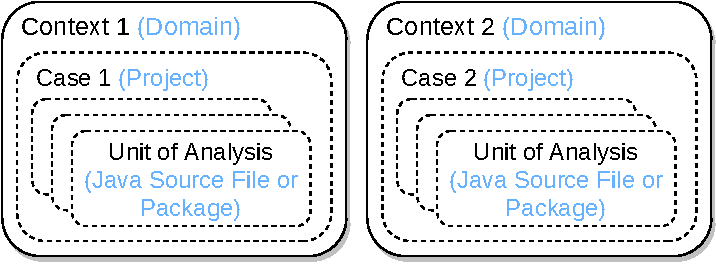
\includegraphics[width=.6\linewidth]{c5/case-design.pdf}
    \caption{The case study design using Runeson et al.'s representation \cite{Runeson2012}.}
    \label{c5:fig:case-design}
\end{figure}

\subsection{Terminology}
In the next sections, we will use the term \emph{change frequency} to indicate the number of times an artifact undergoes any kind of change in a given number of commits.
For example, if an artefact changes in 3 commits out of the 100 considered, its change frequency is $.03$.

The term \emph{change size} refers to the sum of the number of lines of code added, deleted, and/or modified to/from an artefact in a single given commit.
This is commonly referred to as \emph{code churn}.
A formal definition of how we measure changes is provided in Section \ref{c5:sec:data-collection}.

Finally, we note that we use the terms \emph{commit} and \emph{version} interchangeably. Additionally, the term \emph{release} is used when a certain commit/version is explicitly packaged and tagged for public release.

\subsection{Goal and Research Questions}
The goal of this study is to understand the impact of architectural smells on source code changes.
Using the Goal-Question-Metric approach \cite{VanSolingen2002}, the goal can be formulated as follows: 
\begin{quote}
    \itshape
    \textbf{Analyse} changes in source code artefacts \textbf{for the purpose of} understanding the impact of architectural smells \textbf{with respect to} the frequency and size of those changes \textbf{from the point of view of} software developers and architects \textbf{in the context of} open source Java software systems.
\end{quote}
By (Java) source code artefacts we mean both source code files (classes) and source code packages.

The goal can be broken down into three main research questions, as follows.
\begin{itemize}
    \item[\textbf{RQ1}] Do classes and packages with smells change more frequently than classes and packages without smells?
    \begin{itemize}
        \item[\textbf{RQ1a}] Do different smell types have a different impact on frequency of change?
        \item[\textbf{RQ1b}] Does the number of smells have a different impact on frequency of change?
    \end{itemize} 
\end{itemize}
We ask this question to shed some light on the actual relationship between the existence of architectural smells and the \emph{change frequency} of classes and packages.
Such a relationship, in case it exists, confirms that architectural smells' presence correlate with increased maintenance effort, with respect to the frequency of changes of the affected artefacts.

The two sub-questions, RQ1a and RQ1b, further explore the connection between architectural smells and change frequency by looking at how different smell types and multiple smells correlate to changes.
% This research question and its sub-questions have already been answered in a previous study by Khomh et al. \cite{Khomh2009} for code smells with interesting results. Thus it is intriguing to compare architectural smells with code smells regarding their impact.

\begin{itemize}
    \item[\textbf{RQ2}] What is the difference in the change frequency of an artefact before and after a smell is introduced?
\end{itemize}
This question aims at identifying whether the introduction of a smell impacts the \emph{change frequency} of a certain artefact.
More precisely, it provides insights on whether the presence of the smell can be related to an increased change frequency in an affected artefact.
Theoretically, one would expect that the introduction of a smell leads to an increase in the change frequency in (at least some of) the artefacts affected by the smell.
Finally, the results of this research question, in case we do find evidence of such an increase, will strengthen the findings of RQ1.

\begin{itemize}
    \item[\textbf{RQ3}] Is the size of the changes in source code artefacts affected by smells, larger than in non-affected artefacts?
\end{itemize}
This question focuses on the magnitude, or \emph{size}, of the changes made (in terms of added, deleted, and changed lines of code) to the artefacts that are affected by smells. Theoretically, these artefacts should exhibit bigger changes (thus more complex ones) because working on an sub-optimal design is harder and thus requires changing more lines of code to be maintained.
Bigger changes, in most scenarios (e.g. fixing bugs, adding features, refactoring, etc.), mean developers have spent more time to implement them, resulting in a higher amount of interest paid\cite{ElEmam2000, Mockus2000}.

We emphasize that, with these research questions we are \textbf{not seeking} to establish causality between smells and changes by any means, but rather we aim at investigating correlations. This is further explained in the Discussion section.

Finally, a replication package, containing the protocol, the data, the R scripts, and a collection of 14 plots that visualise the data, is available online\footnote{\label{ftn:repl-package}Visit \url{https://doi.org/10.5281/zenodo.4897281} to download the replication package.}.

\subsection{Analysed Projects}
To conduct our study, we selected the thirty-one projects listed in Table \ref{c5:tab:projects}. 
The inclusion criteria used during the selection of the projects were:
\begin{enumerate}
    \item Non-trivial Java projects with at least $10.000$ lines of code in the last commit; 
    \item Actively maintained and used by the community (the Contributors page on GitHub should show a consistently active development\footnote{See for example Accumulo's page \url{https://github.com/apache/accumulo/graphs/contributors} for an example of actively-developed project.});
    \item At least 3 years of active development on GitHub (or similar sites);
\end{enumerate}
During the selection process we also strove to diversify the domains of the included systems as much as possible, as indicated in Table \ref{c5:tab:projects}, as well as to increase as much as possible the period of analysis taken into consideration.
To this end, our dataset contains thirty one projects, with an average period of analysis of 11.5 years, a maximum of 22.1 years, and a minimum of 3.5 years with an average of 126.8 commits analysed per project.
Figure \ref{c5:fig:projects-versions-loc} reports the distribution of the total number of lines of code of the commits analysed for each project.

\begin{table}[]
    \scriptsize
    \centering
    \caption{Demographics of the projects analysed in this study. Note that dates refer to the period of analysis taken into consideration, not age of the system. Additionally, the categories are only indicative.}\label{c5:tab:projects}
      \begin{tabular}{m{1.75cm}|l|l|l|l|l}
      \toprule
      \textbf{Category} & \textbf{Project} & \multicolumn{1}{l|}{\makecell{\textbf{\# Commits} \\ \textbf{analysed}}} & \textbf{1st/last commit} & \multicolumn{1}{l|}{\makecell{\textbf{KLOC 1st-} \\ \textbf{last commit}}} & \textbf{Description}\\
      \midrule

      % Data Storage & Management
      \multirow{6}{1.75cm}{Data storage and Management} & accumulo & 99 & 12-2011/ 11-2019 & 193 - 237 & Data Storage System \\
       & calcite & 81 & 11-2014 / 5-2021 & 109 - 187 & Dynamic Data Management \\
       & cassandra & 136 & 4-2009 / 11-2019 & 36 - 178 & Distrib. NoSQL database \\
       & chukwa & 73 & 10-2008 / 4-2019 & 8 - 31 & Data Collection \\
       & jackrabbit & 155 & 12-2006 / 11-2019 & 94 - 241 & Content Repository \\
       & jackson & 93 & 2-2012 / 11-2019 & 31 - 59 & Data Binding Library \\ \midrule

      % Web  engine and tools
      \multirow{5}{1.75cm}{Web engines and Web Tools} & httpcomp. & 126 & 2-2006 / 10-2019 & 0 - 33 & HTTP Toolset \\
       & jspwiki & 186 & 8-2001 / 11-2019 & 1 - 32 & Wiki Engine \\
       & retrofit & 51 & 6-2015 / 6-2020 & 3 - 10 & Android HTTP client\\
       & spring-boot & 47 & 10-2017 / 5-2021 & 91 - 143 & Spring-based project manager\\
       & struts & 158 & 4-2006 / 11-2019 & 24 - 41 & Web Apps Framework \\\midrule

      % Search engine  
      \multirow{4}{1.75cm}{Search Engines} & elasticsearch & 49 & 7-2015 / 3-2019 & 295 - 614 & Search engine \\
       & jena & 95 & 6-2012 / 11-2019 & 209 - 348 & Semantic Web \\
       & lucene & 173 & 10-2001 / 8-2015 & 5 - 453 & Search Engine \\
       & tika & 144 & 8-2007 / 11-2019 & 2 - 63 & Content Analysis Toolkit \\\midrule

      % CI/CD Tools
      \multirow{5}{1.75cm}{Development Tools} & ant-ivy & 130 & 7-2005 / 11-2019 & 10 - 42 & Dependency Manager \\
       & jenkins & 186 & 12-2006 / 5-2021 & 14 - 125 & Automation server \\
       & jgit & 123 & 11-2009 / 11-2019 & 18 - 113 & Java implementation of Git\\
       & selenium & 132 & 2-2011 / 5-2021 & 2 - 53 & Automation web libraries\\
       & testng & 147 & 9-2006 / 10-2019 & 13 - 59 & Testing Framework \\\midrule

      % Document APIs
      \multirow{3}{1.75cm}{Document Manipulation} & pdfbox & 137 & 8-2008 / 11-2019 & 26 - 82 & PDF Library \\
       & poi & 206 & 3-2002 / 11-2019 & 19 - 99 & MS Office API \\
       & xerces2 & 189 & 1-2000 / 7-2019 & 36 - 116 & XML Library \\\midrule

      % Database APIs
      \multirow{2}{1.75cm}{JDBC Drivers} & druid & 99 & 6-2011 / 11-2019 & 42 - 85 & Alibaba JDBC Library \\
       & pgjdbc & 211 & 9-1997 / 11-2019 & 2 - 30 & PostgreSQL JDBC driver \\\midrule

      % Networking & Messaging
      \multirow{2}{1.75cm}{Networking and Messaging} & activemq & 161 & 1-2006 / 11-2019 & 61 - 177 & Message Server \\
       & mina & 120 & 3-2005 / 6-2019 & 6 - 28 & Network Framework \\ \midrule

      % Game engine
      Game Engine & libgdx & 139 & 4-2010 / 5-2021 & 23 - 222 & Game engine\\ \midrule

      % Data binding
      \multirow{2}{1.75cm}{Data Binding} & fastjson & 104 & 9-2011 /5-4-2021 & 12 - 41 & Alibaba JSON data mapper \\
       & gson & 99 & 9-2008 / 5-2021 & 6 - 10 & Google JSON data mapper\\ \midrule

      Utility & guava & 83 & 1-2010 / 7-2019 & 33 - 117 & Google Core Library \\
      
      \bottomrule
      \end{tabular}%
\end{table}%

\begin{figure}
    \centering
    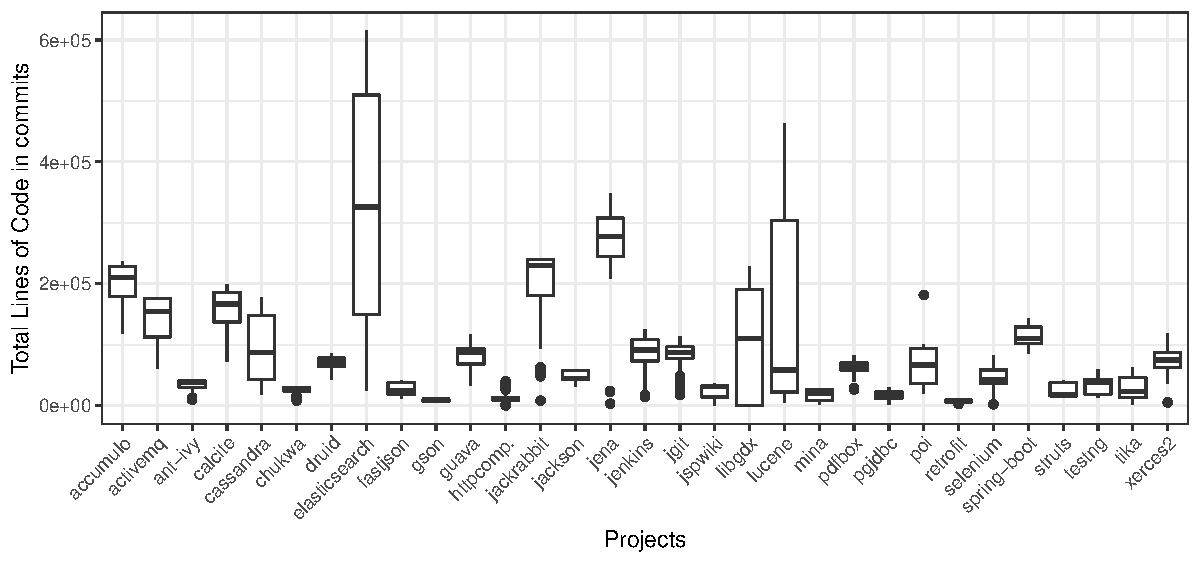
\includegraphics[width=.9\linewidth,clip,trim={0 0.7cm 0 0}]{c5/project-version-loc.pdf}
    \caption{The distribution of the total number of lines of code of each version for each project.} \label{c5:fig:projects-versions-loc}
\end{figure}


\section{Data Collection}\label{c5:sec:data-collection}
For every system $S$ listed in Table \ref{c5:tab:projects} we analysed one commit (or version) $v$ every 4 weeks, from the first commit available in the repository to the latest on the main branch (either master or trunk).
We selected a 4-week-long interval between each commit because we wanted to ensure that the change-related metrics we selected were calculated at a meaningful level of granularity, allowing enough files to change from one commit to the next one.
Such custom intervals were used in similar contexts by previous studies \cite{Nagappan2007,Kouroshfar2015,Arcelli2019b}.
Additionally, a fixed interval between commits, avoids the introduction of bias and ensures the results are consistent across the different release rates of our projects \cite{Kouroshfar2015}. The selection of the 4-week-long interval is further discussed in the Threats to Validity Section.
The change-related data were extracted using \texttt{git diff} between each pair of consecutive commits.
The period of analysis started from the first ever commit available on the repository to the last one available as of May 2021. Next, as part of our data cleaning process, we removed the commits with no changes at the beginning and ending of a project, as these entail inactive leading and trailing periods.


For every artefact $x$, namely class $c$ or package $p$, in each commit $v$ we collected the following \textbf{\emph{independent}} variables: (1) a boolean variable denoting whether $x$ was affected by architectural smells or not, (2) four boolean variables indicating whether a certain type of smell affects $x$, (3) and an integer variable counting the total number of smell instances per smell type that affected it.
We also measure, for every artefact $x$ the changes in the system using a well-established suite of metrics provided by Elish et al. \cite{Elish2013} -- these are the \textbf{\emph{dependant}} variables in our study:
\begin{enumerate}
   \item \textbf{Change Has Occurred (CHO)}. This metric is the basis for calculating the \emph{change frequency} of an artifact. \emph{CHO} measures whether a class $c$, or package $p$, has changed or not in the current commit $v$ with respect to the previous commit $v-1$ in the dataset:
    \begin{align*} 
    CHO_v(c) = \begin{cases}
        1 & \text{if } c \text{ has changed in } v \\
        0 & \text{otherwise}
    \end{cases} &&
    CHO_v(p) = \bigvee_{c \in p}^{p} CHO(c)
    \end{align*} 
    Note that to calculate \emph{CHO} for a package $p$ (i.e. right-most formula) we do a binary sum (i.e. binary \emph{OR}) between all the elements $c$ directly contained in $p$.

    \item \textbf{Percentage of Commits a Class has Changed (PCCC)}. This metric computes the \emph{change frequency} of an artefact using \emph{CHO} and is represented as a percentage to normalise it. The metric was described and used in previous studies \cite{Arvanitou2017,Zhang2013} and is basically the \emph{FRCH} metric defined by Elish et al. \cite{Elish2013} but normalised as a percentage.
    $$PCCC^a_b(x) = \frac{\sum_{v = a}^{b} CHO_r(x)}{b-a} \times 100$$
    where $v$ is the commit for which CHO is computed, and $[a, b]$ is the interval of commit indexes considered.
    Intuitively, this metric counts the number of commits where an artefact has undergone changes and divides it by the number of commits in the period considered.

    \item \textbf{Total Amount of Changes (TACH)}. Also called \emph{change size}, or \emph{code churn}, is the sum of added lines of code (\emph{NAL}), deleted lines (\emph{NDL}), and twice the changed lines (\emph{NCL}) since the last commit\cite{Elish2013} for a given class $c$ or package $p$:
    \begin{align*}
    TACH(c) = NAL(c) + NDL(c) + 2 \times NCL(c) &&   
    TACH(p) = \sum_{c \in p}^{p} TACH(c) 
    \end{align*}
    The calculation of \emph{TACH} for packages is simply the sum of \emph{TACH} for each class $c$ directly contained in $p$.
\end{enumerate}


To collect the data, we used a combination of two tools: \textsc{Arcan} \cite{Arcelli2016} and ASTracker \cite{Sas2019}. \textsc{Arcan} collected the artefacts affected by architectural smells in each selected commit in the history of the systems directly from the source code files.
The output of \textsc{Arcan} is a graph file containing the dependency network of the commit analysed, including the smells detected.
The algorithms used to detect architectural smells are explained in detail by Arcelli et al. in their paper\cite{Arcelli2016}. The detection is based on the software design principles reported by Martin \cite{Martin2018} and Lippert \cite{Lippert2006}.
In short, Cyclic Dependency is detected using a Depth-First Search algorithm that visits all the nodes in the dependency graph while checking which were already visited. 
Unstable Dependency is detected using Martin's Instability metric \cite{Martin2018}: if the \emph{majority} of a package's  dependencies are less stable than itself, then it is marked as an unstable dependency smell.
Hublike Dependency is detected by simply looking at the number of incoming and outgoing dependencies a certain artefact has: if the sum of these dependencies surpasses a certain system-based threshold, then the artefact is marked as a hub.
Finally, God Component is detected using an automatically-calculated variable threshold \cite{Arcelli2015} using the distribution of the total amount of lines of code of the packages in a benchmark of over 100 systems; the packages in the analysed system are then compared with this threshold and the artefacts surpassing it are marked as God Components \footnote{See \url{https://fse.studenttheses.ub.rug.nl/19603/} for more details.}.

\textsc{Arcan}'s results were validated in different studies. A first validation of the results of \textsc{Arcan} was performed on two open source projects with a precision of 100\% \cite{Arcelli2016}. 
Next, the results of \textsc{Arcan} were also validated in an industrial setting by two different studies: first on industrial C/C++ projects obtaining 50\% precision \cite{Martini2018} and then on industrial Java projects obtaining 70\% precision \cite{Arcelli2020}.
The precision metric was chosen as the main indicator of \textsc{Arcan}'s performance because the true positive rate was found to be the main concern for developers during the mentioned studies.

The second tool we used, ASTracker, computed the above-mentioned change metrics and identified the elements affected by each smell.
ASTracker's main feature is to track architectural smells from one version to the next (i.e. link the same instances detected in two adjacent versions), but for this study it was only used to calculate the change metrics as stated above. To guarantee the correctness of the implementation of the change metrics, we used thorough unit testing.

At last, the Peregrine high performance computing cluster, offered by the University of Groningen, provided the computational power necessary to carry out the whole data collection process.

\section{Data analysis}\label{c5:sec:data-analysis}
\subsection{Controlling for size}\label{c5:sec:data-analysis-size}
Changes to source code files are intuitively more frequent in files of greater size (i.e. more lines of code). In fact, source code size has been empirically found to interfere with the actual findings in several cases \cite{ElEmam2001,Zhou2009}. Thus, source code size is a confounding factor in our analysis that could skew the results unpredictably and obfuscate the impact of smells on change frequency and size.
To mitigate this threat, as already mentioned in the Introduction and Related Work sections, the data analysis will include controlling for size. Specifically, we will analyse the data both by considering all artefacts (without controlling for source code size) and by grouping the artefacts (either classes or packages) into four size groups, based on their effective lines of code (LOC). This way we can compare how smells impact files of similar size.
The groups are defined as follows: Small = $[1, Q_1)$, Medium-Small (M-Small) = $[Q_1, Q_2)$, Medium-Large (M-Large) = $[Q_2, Q_3)$, and Large = $[Q_3, Q_4)$, where $Q_1$, $Q_2$, $Q_3$, $Q_4$ are the first, second, third, and fourth quartiles respectively of the distribution of the LOC of classes (or packages, when working with smells affecting packages) in a given project. This means that these values differ for each project. Table \ref{c5:tab:quartiles-loc} shows the quartiles of the LOC distribution in the whole data set.


\begin{table}[]
    \caption{Distribution of the Lines Of Code metric in classes and packages in the whole data set.}
    \centering
    \label{c5:tab:quartiles-loc}
    \begin{tabular}{@{}llllll@{}}
    \toprule
            & \textbf{0\%} & \textbf{25\% ($Q_1$)} & \textbf{50\% ($Q_2$)} & \textbf{75\% ($Q_3$)} & \textbf{100\% ($Q_4$)} \\ \midrule
    Class   & 1   & 10        & 27        & 77        & 14990 \\
    Package & 1   & 549       & 1340      & 2976      & 59074 \\ \bottomrule
    \end{tabular}
\end{table}

This approach was proposed by Aniche et al. in a previous study \cite{Aniche2018}. We adopted it as it  allows us to compare smelly and non-smelly artefacts with comparable size.
This method guarantees that all four groups have the same number of files, which is an important prerequisite to ensure that the results of the study are not skewed. Indeed, if we were to partition the files, for example, with a range of 45 LOC per group, the resulting small group (0-45 LOC) would have 200K+ artefacts, whereas the others just a few thousands. This imbalance would greatly affect the outcome. 


\subsection{RQ1 -- Do classes and packages with smells change more frequently than classes and packages without smells?}
For this RQ we statistically analyse the significance of the association between changes in affected and non-affected artefacts.
The Fisher's exact test of independence \cite{Sheskin2007} is performed on two categorical variables: in our case, these variables are CHO and whether this artefact is affected by a smell.
The input to the test is a contingency table where all the possible values of the two (categorical) variables are listed on the rows and columns of the table respectively. 
The null and alternative hypotheses of the tests (one test for each 4-month-long period considered) are:
\begin{itemize}
    \item \textbf{Null hypothesis} $H^{RQ1}_0$: artefacts affected by smells are \textit{equally} likely to be subject to changes than artefacts not affected by smells ($\pi_1 = \pi_2$)
    \item \textbf{Alt. hypothesis} $H^{RQ1}_1$: artefacts affected by smells are more likely to be subject to changes than artefacts not affected by smells ($\pi_1 > \pi_2$)
\end{itemize}
where $\pi_1$ and $\pi_2$ represent the proportions of the two categories with respect to the overall population.

To ensure the test is \emph{supported}, we need to make sure that the proportions in the contingency tables used to run the tests are not excessively unbalanced towards one category. Contingency tables are likely to be unbalanced if the time period is too small because only limited changes can happen in a certain amount of time and that time can not be enough to determine whether the correlation is present or not.
In other words, given that there are more non-changing files than changing files, a period of 1 month is likely to be insufficient for enough files to change.
Thus we aggregated our data to a 4-month granularity (rather than 1-month); this is approximately the average release rate we mined from the Git tags of our projects. We call these ``versions'' \emph{pseudo-releases}.
Thus, for each pseudo-release $v$, we test for the null-hypothesis, namely, whether there is no statistical difference in the proportions of changes for artefacts affected and not affected by architectural smells. 
This analysis will include all types of smells, both at class and package level, detected by \textsc{Arcan}.

The next step is to compare the percentages of pseudo-releases that do show a significant difference (accepting $H^{RQ1}_1$) and the pseudo-releases that do not show any significant difference (accepting $H^{RQ1}_0$), which will allow us to answer RQ1.
Note that we opted to perform one test per commit per project, rather than one test per project, to ensure that the imbalance in changes detected is not the result of a few change hotspots throughout the history of the system, but rather a more constant phenomenon.
The confidence level used for this test and all the following tests is equal to $\alpha = .05$.

\subsubsection{RQ1a -- Do different smell types have a different impact on frequency of change?}\label{c5:sec:rq1a-analysis}
In order to answer RQ1a, we used a logistic regression model \cite{Sheskin2007}. This kind of model allows to predict the value of a binary dependant variable given a set of multiple independent variables. 
Moreover, it can be exploited to compute the effect size between the dependant variable and each independent variable, to identify which variable influences the outcome.
In this case, we chose the CHO metric (see Section \ref{c5:sec:data-collection}) as dependant variable and the number of smell instances of each smell type $t$ as independent variables.

The hypotheses of this analysis are:
\begin{itemize}
    \item \textbf{Null hypothesis} $H^{RQ1a}_0$: the type of smells does not have an impact on the occurrence of changes of artefacts
    \item \textbf{Alt. hypothesis} $H^{RQ1a}_1$: the type of smells does have an impact on the occurrence of changes of artefacts.
\end{itemize}
The analysis was performed individually for each 4-month commit period, for all projects. Then, for each type of smell we counted the number of times that the $p$-values obtained by the logistic regression were significant.

\subsubsection{RQ1b -- Does the number of smells have a different impact on frequency of change?}
For RQ1b we used the non-parametric Mann-Whitney statistical test to check whether the average number of smells per commit in artefacts that do not change and in artefacts that do change is statistically similar.
Formally, we calculate
\begin{align*}
    changed(v) = \sum_x^{C_v}\frac{n_v(x)}{|C_v|} & & unchanged(v) = \sum_x^{U_v}\frac{n_v(x)}{|U_v|}
\end{align*}
%$$ changed(v) = \sum_x^{C_v}\frac{n_v(x)}{|C_v|}$$
%$$ unchanged(v) = \sum_x^{U_v}\frac{n_v(x)}{|U_v|}$$

where $C_v$ is the set of artefacts $x$ that changed in commit $v$, $U_v$ is the set of unchanged artefacts, and $n_v(x)$ counts the number of smells $x$ has in $v$.
 
The hypotheses for this analysis are:
\begin{itemize}
    \item \textbf{Null hypothesis} $H^{RQ1b}_0$: the number of smells in artefacts that do not change is equal to the number of smells in artefacts that do change ($\mu_{unchanged} = \mu_{changed} $)
    \item \textbf{Alt. hypothesis} $H^{RQ1b}_1$: the number of smells in artefacts that do not change is \emph{less} than the number of smells in artefacts that do change  ($\mu_{unchanged} < \mu_{changed} $).
\end{itemize}
with $\mu$ representing the mean of the populations (changed and unchanged).
Additionally, to further reinforce the findings we also check whether there is any correlation (using Spearman's $\rho$) between the number of smells an artefact is affected by and the number of changes or their size.

\subsection{RQ2 -- What is the difference in the change frequency of an artefact before and after a smell is introduced?}\label{c5:sec:rq2-analysis}
The analysis for this research question will look at the PCCC metric of a certain artefact before and after a smell is introduced in that element. We then aggregate the data per project and perform a Wilcoxon Signed-Ranks test \cite{Sheskin2007} for each project.

Formally, for every artefact $x$ affected by a smell in the lifetime of a system $S$ we compute 
$$d_S(x) = PCCC_{after}(x) - PCCC_{before}(x)$$
where $PCCC_{before}(x) = PCCC^i_k(x)$ and $PCCC_{after}(x) = PCCC^k_j(x)$ with $i$ being the commit index where $x$ first appeared, $k$ where it was first affected by a smell, and $j$ when it was last affected by a smell, or the final commit.
Artefacts with either a before or after window smaller than 5 commits were filtered out to avoid skewed data.
The values assumed by $d_S$ for the selected artefacts from $S$ are used as input for the test.

The hypotheses for this test are:
\begin{itemize}
    \item \textbf{Null hypothesis} $H^{RQ2}_0$: the change frequency of artefacts before and after a smell is introduced is the same ($\theta_{d_S} = 0$)
    \item \textbf{Alt. hypothesis} $H^{RQ2}_1$: the change frequency of artefacts after a smell is introduced is greater than before ($\theta_{d_S} > 0$). 
\end{itemize}
where $\theta$ represents the true median of the underlying population.
Additionally, using the Shapiro–Wilk test, we also test for the normality of $d_S$ to ensure we chose the appropriate statistical test.

\subsection{RQ3 -- Is the size of the changes in source code artefacts affected by smells, larger than in non-affected artefacts?}
For this RQ we want to investigate if there is a significant difference in the \emph{variance} of the size of the changes in affected versus non-affected artefacts in each commit analysed.
We look at the variance because the majority of commits have a relatively small change size, whereas few commits (e.g.  the pull requests) have a very large change size.

To determine whether there is a significant difference in these two groups (smelly vs non-smelly), we perform a Brown-Forsythe test for the homogeneity of variance \cite{Sheskin2007}.

For each commit $v$ we compute the aggregate change size (TACH metric) of changing artefacts by averaging all the change sizes for that commit.
Formally:
\begin{align*}
    smelly(v)  = \sum_{x}^{A_v} \frac{TACH(x)}{|A_v|} & & & clean(v) = \sum_{x}^{N_v} \frac{TACH(x)}{|N_v|}
\end{align*}
where $A_v$ is the set of affected artefacts in a commit $v$, and $N_v$ the non-smelly artefacts. Note that we use the term ``clean'' to indicate \textbf{non-smelly} artefacts for conciseness.

Next, we test the following hypotheses on those two variables for each project:
\begin{itemize}
    \item \textbf{Null hypothesis} $H^{RQ3}_0$: the variance in change size is equal in affected and clean artefacts by smells ($\sigma^2_{smelly} = \sigma^2_{clean}$)
    \item \textbf{Alt. hypothesis} $H^{RQ3}_1$: the variance in change size is not equal in affected and clean artefacts ($\sigma^2_{smelly} \ne \sigma^2_{clean}$)
\end{itemize}
where $\sigma^2_{smelly}$ and $\sigma^2_{clean}$ represent the true variance in the underlying populations.


\section{Results}\label{c5:sec:results}
\subsection{Relation between change frequency and smelly artefacts (RQ1)}
The results of the Fisher's tests (main question of RQ1) performed on each 4-month period of the thirty-one systems analysed are pretty straightforward when not controlling for size.
Figure \ref{c5:fig:rq1-results} reports in detail the number of 4-month periods (or pseudo-releases) where the null hypothesis was accepted, rejected, or the test was unsupported by the data.
The proportion of smelly artefacts that change is consistently higher than non-smelly artefacts that change in $82$\% of the total 4-month periods analysed in most of the projects (rejecting $H^{RQ1}_0$). In other words, \textbf{artefacts with smells do change more frequently}. For the remaining $18$\%, if we remain conservative and assume that the $11.5$\% of the unsupported tests are accepted, the smelly and non-smelly artefacts are equally likely to change (accepting $H^{RQ1}_0$).
Note that the unsupported tests are usually the ones corresponding to the pseudo-releases in the early phases of the project with a relatively little number of smells and/or changes.
We also note that these percentages hold for the majority of the projects, with six exceptions: Elasticsearch, Jena, HTTP-components, Guava, Retrofit, and Spring-boot.
These projects exhibit the opposite scenario, with more than $50$\% of the pseudo-releases featuring changes in non-smelly artefacts (neither accepting nor rejecting $H^{RQ1}_0$).
This can be at least partially explained in all six cases: they either have a very low density of smells (HTTP-components and Retrofit) or the actual proportion of smelly components that change is lower (up to 10 times) than non-smelly components that change (Elasticsearch, Guava and Jena).
\begin{figure}[t]
    \centering
    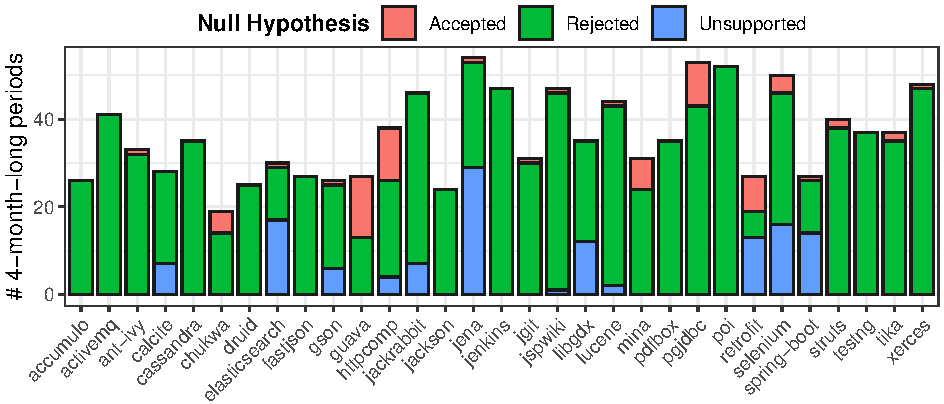
\includegraphics[width=.8\linewidth]{c5/rq1.pdf}
    \caption{Results of the Fisher's test for each project (Averages: Accepted: $6.5$\%; Rejected: $82.1$\%; Unsupported: $11.4$\%).}\label{c5:fig:rq1-results}
\end{figure}

When adjusted for size (using the lines of code - see Section \ref{c5:sec:data-analysis-size}), the results depicted in Table \ref{c5:tab:rq1-results} show that 
for \emph{Medium-Large} and \emph{Large} artefacts the null hypothesis $H^{RQ1}_0$ was rejected $66.1$\% and $78.9$\% of the times on average across all projects, respectively.
For \emph{Small} and \emph{Medium-Small} artefacts, percentages drop to $30.2$\% and $45.4$\%, respectively.
In total,  $H^{RQ1}_0$ was rejected $55.7$\% of the times and accepted $30.2$\%, while in the remaining $14.1$\% of times, the analysis was unsupported.

Ultimately, the results controlled for size do not deviate too much from the uncontrolled ones, but allow us to discern that \textbf{the larger the file, the more an artefact is likely to change if affected by a smell}.

\begin{table}
    \footnotesize
    \centering
    \caption{Percentages of rejected $H^{RQ1}_0$ per project by size group. (Averages: Accepted: $33.6$\%; Rejected $59.1$\%; Unsupported: $7.3$\%)}\label{c5:tab:rq1-results}
    \begin{tabular}{l|r|r|r|r}
        \toprule
        \multirow{2}{*}{\textbf{Project}} & \multicolumn{4}{c}{\textbf{\% P-value $< .05$}} \\
        & \textbf{Small} & \textbf{Med.-Small} & \textbf{Med.-Large} & \textbf{Large} \\
        \midrule
        accumulo & \databar{38.5} & \databar{65.4} & \databar{96.2} & \databar{100.0} \\
        activemq & \databar{78.0} & \databar{65.9} & \databar{100.0} & \databar{100.0} \\
        ant-ivy & \databar{57.6} & \databar{57.6} & \databar{90.9} & \databar{100.0} \\
        calcite & \databar{67.9} & \databar{64.3} & \databar{75.0} & \databar{71.4} \\
        cassandra & \databar{74.3} & \databar{94.3} & \databar{100.0} & \databar{100.0} \\
        chukwa & \databar{0.0} & \databar{31.6} & \databar{42.1} & \databar{63.2} \\
        druid & \databar{40.0} & \databar{84.0} & \databar{96.0} & \databar{100.0} \\
        elasticsearch & \databar{30.0} & \databar{43.3} & \databar{43.3} & \databar{43.3} \\
        fastjson & \databar{7.4} & \databar{33.3} & \databar{85.2} & \databar{88.9} \\
        gson & \databar{3.8} & \databar{0.0} & \databar{30.8} & \databar{69.2} \\
        guava & \databar{37.0} & \databar{0.0} & \databar{25.9} & \databar{29.6} \\
        httpcomp. & \databar{2.6} & \databar{13.2} & \databar{36.8} & \databar{39.5} \\
        jackrabbit & \databar{15.2} & \databar{69.6} & \databar{84.8} & \databar{84.8} \\
        jackson & \databar{33.3} & \databar{95.8} & \databar{100.0} & \databar{100.0} \\
        jena & \databar{9.3} & \databar{29.6} & \databar{38.9} & \databar{44.4} \\
        jenkins & \databar{44.7} & \databar{72.3} & \databar{95.7} & \databar{100.0} \\
        \bottomrule
    \end{tabular}
    \quad
    \begin{tabular}{l|r|r|r|r}
        \toprule
        \multirow{2}{*}{\textbf{Project}} & \multicolumn{4}{c}{\textbf{\% P-value $< .05$}} \\
        & \textbf{Small} & \textbf{Med.-Small} & \textbf{Med.-Large} & \textbf{Large} \\
        \midrule
        jgit & \databar{48.4} & \databar{77.4} & \databar{96.8} & \databar{96.8} \\
        jspwiki & \databar{31.9} & \databar{70.2} & \databar{68.1} & \databar{89.4} \\
        libgdx & \databar{8.6} & \databar{28.6} & \databar{78.3} & \databar{100.0} \\
        lucene & \databar{38.6} & \databar{47.7} & \databar{56.8} & \databar{75.0} \\
        mina & \databar{25.8} & \databar{12.9} & \databar{38.7} & \databar{67.7} \\
        pdfbox & \databar{54.3} & \databar{77.1} & \databar{94.3} & \databar{100.0} \\
        pgjdbc & \databar{24.5} & \databar{35.8} & \databar{64.2} & \databar{79.2} \\
        poi & \databar{36.5} & \databar{55.8} & \databar{92.3} & \databar{100.0} \\
        retrofit & \databar{0.0} & \databar{0.0} & \databar{3.7} & \databar{11.1} \\
        selenium & \databar{18.0} & \databar{36.0} & \databar{40.0} & \databar{62.0} \\
        spring & \databar{14.8} & \databar{3.7} & \databar{25.9} & \databar{44.4} \\
        struts & \databar{40.0} & \databar{32.5} & \databar{85.0} & \databar{95.0} \\
        testng & \databar{5.4} & \databar{5.4} & \databar{37.8} & \databar{100.0} \\
        tika & \databar{13.5} & \databar{51.4} & \databar{70.3} & \databar{91.9} \\
        xerces2 & \databar{35.4} & \databar{52.1} & \databar{56.2} & \databar{97.9} \\ \midrule
        \textbf{Avrg.} & \databar{30.2} & \databar{45.4} & \databar{66.1} & \databar{78.9} \\
        \bottomrule
    \end{tabular}
\end{table}

\paragraph{RQ1a}
The aim of answering RQ1a was to understand if the specific type of the smells affecting the artefacts has an impact on the occurrence of changes. Table~\ref{c5:tab:rq1a-results} introduces the results of the multinomial logistic regression model.
For each type of smell, it shows the proportion of the 4-month-long periods where the null hypothesis was rejected.
A large number of rejected instances means that the given type of smell has a significant effect on the dependant variable of the regression model, that is the \emph{occurrence of changes}.
The table reports all the statistically significant rates where a variable was considered relevant in the prediction of a change. Each column is a different model calibrated for that size group (or using all files in the case of `Uncontrolled').
We first notice that all the variables exhibit an increase in significance as we look at size groups of larger files.
There seems to be no particular smell type, perhaps only excluding Hublike Dependency, that provides a clear contribution to the regression model over the other types.

The results imply that, in most cases, HL is the smell that contributes the most to changes, however, there is no sufficient evidence to affirm that there is a clear distinction between different types of smell.
Thus, we conclude that we accept $H^{RQ1a}_0$ and affirm that \textbf{there is \emph{no significant difference} in the prediction power of different smell types on source code changes}.

\begin{table}
    \footnotesize
    \centering
    \caption{Results of the multinomial logistic regression in percentage of commits a variable was statistically significant in predicting a change (Rejecting $H^{RQ1a}_0$).}\label{c5:tab:rq1a-results}
    \begin{tabular}{l|r|r|r|r|r}
        \toprule
        \multirow{2}{*}{\textbf{Variable}} & \multicolumn{5}{c}{\textbf{Commits \% when variable is significant}} \\
        & \textbf{Small} & \textbf{Med.-Small} & \textbf{Med.-Large} & \textbf{Large} & \textbf{Uncontrolled} \\
        \midrule
        Cyclic Dependency   & \databar{12.2} & \databar{14.1} & \databar{20.2} & \databar{29.1} & \databar{39.7} \\
        Unstable Dependency & \databar{8.3}  & \databar{14.6} & \databar{20.6} & \databar{32.4} & \databar{29.7} \\
        Hublike Dependency  & \databar{22.1} & \databar{22.3} & \databar{26.7} & \databar{44.6} & \databar{51.9} \\
        God Component       &  --            & --             & --             & \databar{30.5} & \databar{38.5} \\
        %Lines Of Code  & \databar{20.0} & \databar{28.8}  & \databar{39.7} & \databar{62.4} & \databar{83.5} \\
        \bottomrule
    \end{tabular}
\end{table}

\paragraph{RQ1b}
Furthermore, for RQ1b, we tested whether the number of smells (including 0) affecting an artefact is an important variable contributing to its change frequency.
The test results, depicted in Figure \ref{c5:fig:rq1b-test} show that in all projects, but two (Guava and Pgjdbc), the average number of smells in changing artefacts is statistically higher than in non-changing artefacts (rejecting $H^{RQ1b}_0$) when not controlling for size.
If we consider the different size groups, the rejection rate is higher in the larger ones, whereas in the \emph{Small} group we reject $H^{RQ1b}_0$ only twice. Additionally, larger size groups also have a larger Cliff's Delta coefficient with 31 tests having $\delta > .5$ in the Large and M-Large groups against the 3 in the M-Small and Small groups, highlighting the difference in magnitude between the values of the two variables tested.

To better grasp the contrast in smell density between changing and non-changing artefacts in different size groups, Figure \ref{c5:fig:rq1b-density} plots the density (i.e. \# commits) of the (average) number of smells of these two categories.
In the figure, one can see how the average number of smells in changing and non-changing artefacts varies in the commits in our data set. When no smells affect an artefact (leftmost side of the plot), in several commits, only the smaller files change. But looking at the Medium-Large and Large files, we observe both curves shifting in shape and moving towards the right of the plot, with the changing artefacts curve growing larger and distantiating itself from the non-changing artefacts curve.
This means that \textbf{for artefacts with more smells, the larger they are, the more likely they are to change}.

Figure \ref{c5:fig:rq1b-numsmells-size-freq} shows how the change frequency varies by the number of smells affecting an artefact, with different colours representing different projects. 
As it can be noted, there is a steep increase in the number of changes as the number of smells increases from 0 to 15, before stabilizing and slightly growing towards the end of the plot\footnote{For reference, the right-most project in yellow-ish/ocra is Cassandra. Per-project plots are available in the replication package.}. 
The Spearman statistical correlation tests show that: 8 projects show a strong ($\rho \ge .7$) positive correlation; 7 show a moderate ($.5 \le \rho < .7$) positive correlation; 5 projects have a weak ($.3 \le \rho < .5$) correlation; for 2 projects there is little-to-no correlation ($ \rho <.3 $); and for the remaining 9 projects $p > .05$.

In summary, \textbf{the more smells affecting an artefact, the higher the change frequency for that artefact}. 

\begin{figure}
    \centering
    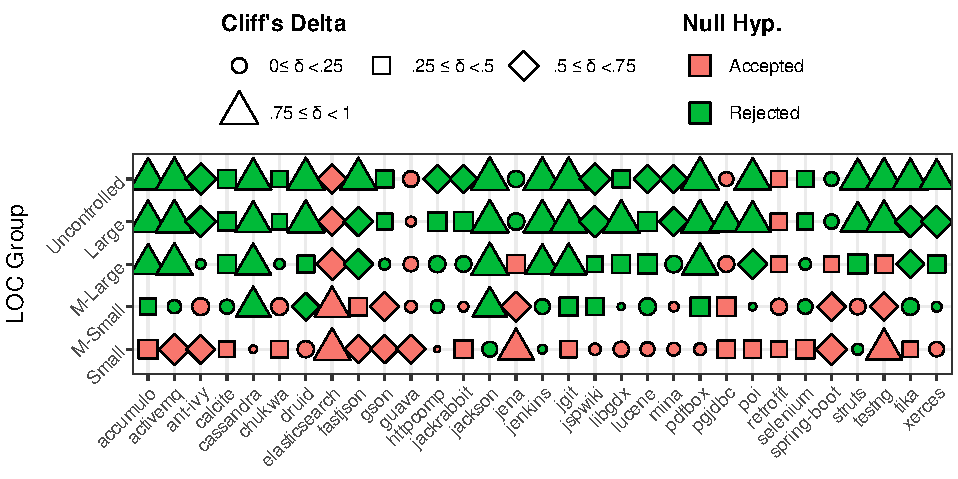
\includegraphics[width=.9\linewidth]{c5/rq1b-test.pdf}
    \caption{Mann-Whitney tests testing $H^{RQ1b}_0$ by size groups.} \label{c5:fig:rq1b-test}
\end{figure}

\begin{figure}
    \centering
    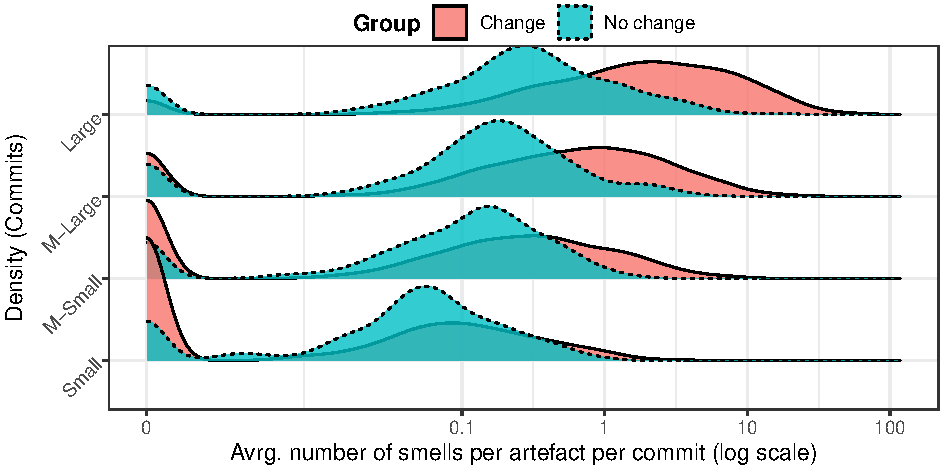
\includegraphics[width=.8\linewidth]{c5/rq1b.pdf}
    \caption{Average number of smells in changing/not-changing artefacts in all the analysed commits by size groups.} \label{c5:fig:rq1b-density}
\end{figure}
granularities
\begin{figure}%
    \centering
    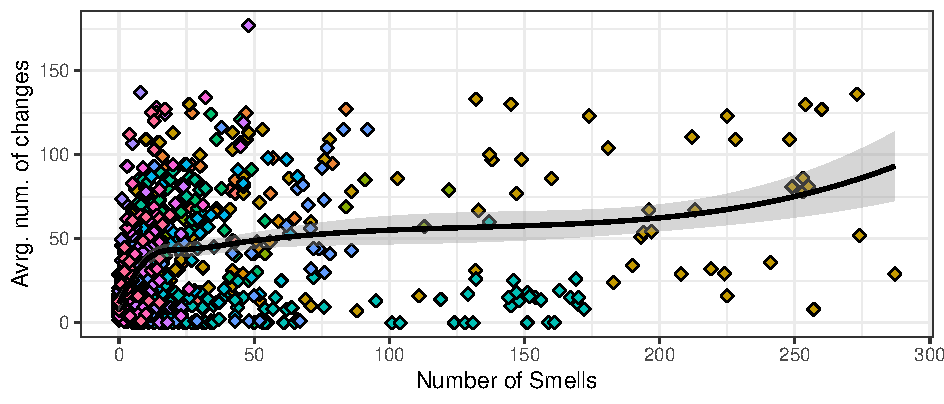
\includegraphics[width=.8\textwidth]{c5/rq1b-numOfChanges.pdf}
    \caption{Average change frequency by number of smells per project (colour-coded). LOESS regression curve shows the trend.}%
    \label{c5:fig:rq1b-numsmells-size-freq}%
\end{figure}

\subsection{Impact on change frequency after the introduction of a smell (RQ2)}
Whereas the results of RQ1 hint that changes are more likely, and more frequent, in smelly artefacts, they do not tell us anything about the effects of the introduction of a smell on the change frequency of a particular artefact throughout its lifetime.
This particular aspect is considered and tested by RQ2 through a series of Wilcoxon Signed-Ranks tests; this was confirmed to be suitable in this case because most of the projects have their $d_S$  (as defined in Section \ref{c5:sec:rq2-analysis}) function not normally distributed.
Note that we do not control for size for this RQ because this is a temporal analysis, thus there is no way to establish exactly which size category one artefact belongs to, as the LOC fluctuate over time.
The results, presented in Table \ref{c5:tab:rq2-results}, indicate that for 16 projects ($57.1\%$) there is an increase in the frequency of changes (in the PCCC metric, to be precise) after a smell is introduced. For 12 projects ($42.9\%$) instead, the opposite holds and more changes happen before the introduction of the smell. Finally, 3 projects did not contained enough samples and were ignored.

We can further inspect the distribution of $d_S$ in Figure \ref{c5:fig:rq2-density}, where we can see how the distribution of changes to the artefacts are skewed either towards the ``before'' or ``after'' the introduction of a smell side, depending on the project. Therefore, we can conclude that, \textbf{in some cases, the introduction of an architectural smell has increased the frequency of changes in the affected component}. We offer a potential explanation for the 12 projects (skewed towards the ``before'' part) that do not conform to this trend in the Discussion section, but we would like to note that 9 of the 16 projects for which we rejected the null hypothesis had $n \le 30$, whereas the accepted ones only had 6.
This means that the tests were likely accepted because of an insufficient number of samples.


\begin{table}[]
    \footnotesize
    \centering
    \caption{Wilcoxon Signed-Ranks results and the sample size (\# of artefacts) for the test ($H^{RQ2}_0$ rejected in bold). (Total: Accepted: $42.9\%$; Rejected: $57.1\%$). }\label{c5:tab:rq2-results}
    \begin{tabular}{l|r|l|r}
        \toprule
        \textbf{Project} & \textbf{P-value} & \textbf{Null Hyp.} & \textbf{Obs.}\\
        \midrule
        accumulo & $ 0.50 $ & Accepted & 11\\
        activemq & $<$ $\textbf{.01}$ & \textbf{Rejected} & 120\\
        ant-ivy & $<$ $\textbf{.01}$ & \textbf{Rejected} & 64\\
        calcite & $<$ $\textbf{.01}$ & \textbf{Rejected} & 75\\
        cassandra & $ 0.30 $ & Accepted & 178\\
        chukwa & $<$ $\textbf{.01}$ & \textbf{Rejected} & 17\\
        druid & $ 0.61 $& Accepted & 47\\
        elasticsearch & $ \textbf{0.04} $& \textbf{Rejected} & 28\\
        fastjson & $ 0.83 $& Accepted & 31\\
        gson & $ 0.50 $& Less than 10 obs. & 5\\
        guava & $<$ $\textbf{.01}$ & \textbf{Rejected} & 34\\
        httpcomp. & $<$ $\textbf{.01}$ & Less than 10 obs. & 9\\
        jackrabbit & $<$ $\textbf{.01}$ & \textbf{Rejected} & 82\\
        jackson & $ 0.28 $& Accepted & 12\\
        jena & $ 0.86 $& Accepted & 11\\
        jenkins & $<$ $\textbf{.01}$ & \textbf{Rejected} & 178\\
        \bottomrule
    \end{tabular}
    \quad
    \begin{tabular}{l|r|l|r}
        \toprule
        \textbf{Project} & \textbf{P-value} & \textbf{Null Hyp.} & \textbf{Obs.}\\
        \midrule
        jgit & $<$ $\textbf{.01}$ & \textbf{Rejected} & 42\\
        jspwiki & $<$ $\textbf{.01}$ & \textbf{Rejected} & 59\\
        libgdx & $ 0.30 $& Accepted & 98\\
        lucene & $<$ $\textbf{.01}$ & \textbf{Rejected} & 220\\
        mina & $<$ $\textbf{.01}$ & \textbf{Rejected} & 22\\
        pdfbox & $<$ $\textbf{.01}$ & \textbf{Rejected} & 103\\
        pgjdbc & $ 0.07 $& Accepted & 23\\
        poi & $ 0.25 $& Accepted & 36\\
        retrofit & $ \textbf{0.04} $& Less than 10 obs. & 4\\
        selenium & $ \textbf{0.03} $ & \textbf{Rejected} & 16\\
        spring-boot & $ \textbf{0.02} $& \textbf{Rejected} & 25\\
        struts & $ 0.05 $& Accepted & 13\\
        testng & $ 0.97 $& Accepted & 15\\
        tika & $ 0.17 $& Accepted & 33\\
        xerces2 & $<$ $\textbf{.01}$ & \textbf{Rejected} & 86\\
        & \\
        \bottomrule
    \end{tabular}
\end{table}

\begin{figure}%
    \centering
    \subfloat{{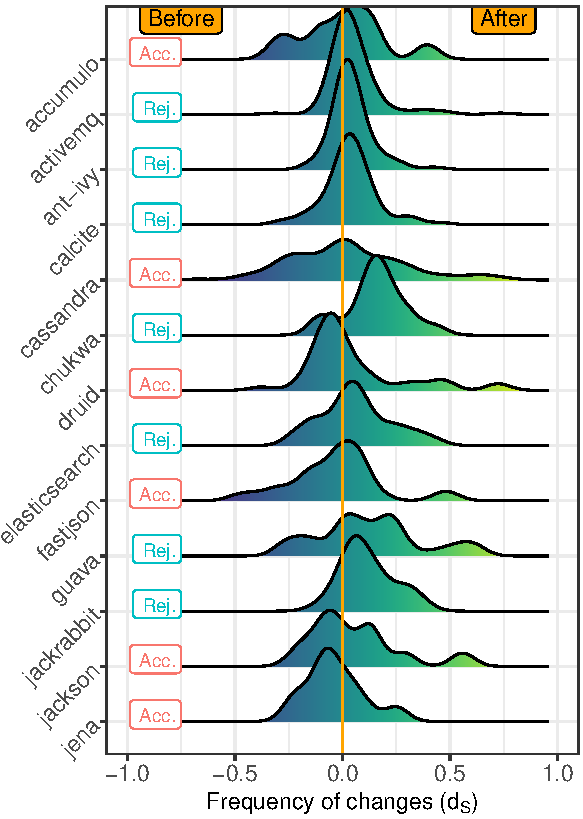
\includegraphics[width=.4\textwidth]{c5/rq2-group1} }}%
    \qquad
    \subfloat{{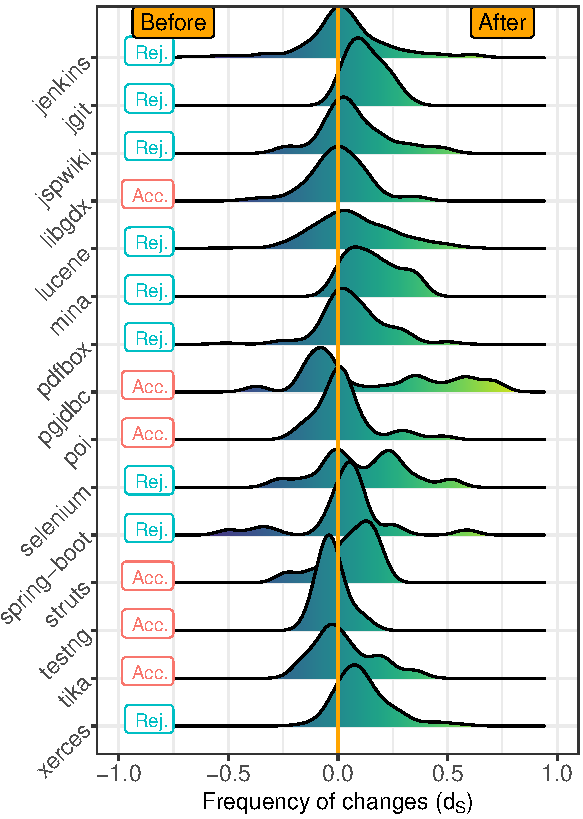
\includegraphics[width=.4\textwidth]{c5/rq2-group2} }}%
    \caption{Density of PCCC before and after the introduction of a smell ($d_S$ function).}%
    \label{c5:fig:rq2-density}%
\end{figure}

\subsection{Comparison of magnitude of changes in smelly and non-smelly artefacts (RQ3)}
For this last question, when testing the null hypothesis $H^{RQ3}_0$ on all projects, without adjusting for the size of the artefacts, we reject it for all of them -- meaning that change size (TACH metric) in artefacts affected by smells has a consistently higher variance than the non-smelly ones.
However, when controlling for the size of the affected artefacts, a different picture emerges.
The results are presented in Figure \ref{c5:fig:rq3-test}. 
Smaller classes and packages do not exhibit this pattern as consistently as the larger ones do; in fact, in \emph{Small} artefacts we note the opposite in the majority of the projects.
For \emph{Large}, \emph{M-Large}, and \emph{M-Small} artefacts the results are consistent in rejecting the null hypothesis $H^{RQ3}_0$.
This can be further visualised in Figure \ref{c5:fig:rq3-violinplots}, where the violin plots of the average change size of smelly and non-smelly artefacts in the analysed commits can be visually compared for each size group. The more elongated the shape of the violin, the larger the variance in the corresponding group.
By observing this figure, we note that the change size in smelly artefacts tends to increase (the violin shifts upwards) as the size of the artefacts increases. In stark contrast, the violin shapes of the non-smelly group are surprisingly similar across the four different groups; this contrast highlights the impact of smells on affected artefacts w.r.t. change size. 

Hence, both visual analysis and statistical tests converge to the same conclusion that \textbf{smelly artefacts undergo changes of higher magnitude than non-smelly artefacts, especially in larger artefacts}.
More precisely, smelly artefacts have an average change size (TACH) across all the projects of 1608, whereas non-smelly artefacts settle at 109. The difference is one order of magnitude higher in smelly artefacts; we note that the smelly artefacts also have a higher variance.

\begin{figure}
    \centering
    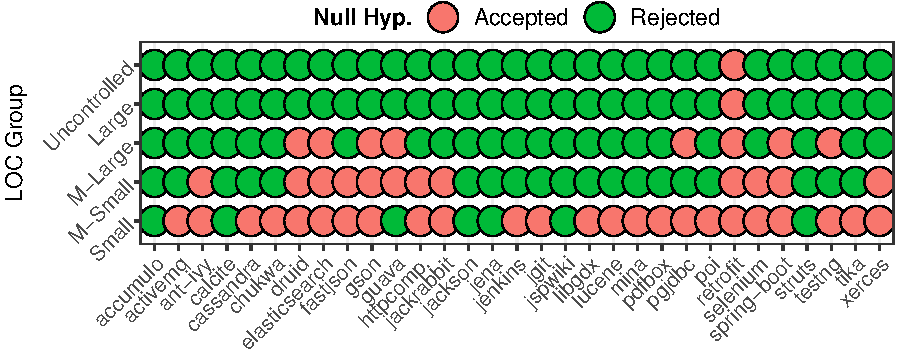
\includegraphics[width=.9\linewidth]{c5/rq3-test.pdf}
    \caption{Brown-Forsythe tests results by size groups for $H_0^3$.}\label{c5:fig:rq3-test}
\end{figure}

\begin{figure}
    \centering
    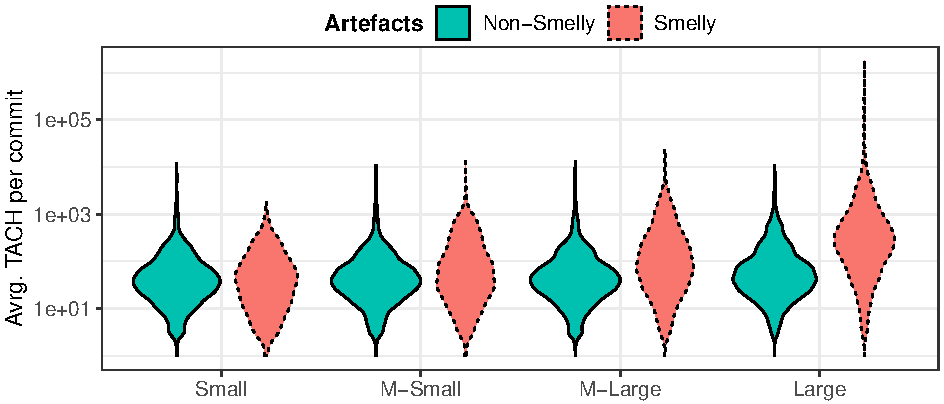
\includegraphics[width=.9\linewidth]{c5/rq3.pdf}
    \caption{Violin plots of the distribution of the average change size (TACH metric) in the analysed commits grouped by  smelly and non-smelly artefacts (log scale).}\label{c5:fig:rq3-violinplots}
\end{figure}


\section{Discussion}\label{c5:sec:discussion}
In the following section we discuss and elaborate on the results presented above.

From the obtained results, we have empirically confirmed that architectural smells (at least the ones considered for this study), exhibit a \emph{correlation} with the \emph{change frequency} and \emph{change size} of the artefacts they affect, and especially the larger artefacts.
As stated previously, our goal was to seek and establish \emph{correlation}, rather than \emph{causality}.

The results from RQ1 show that artefacts affected by at least one smell exhibit more changes than artefacts without smells. We also saw that as the number of smells increases, so does the likelihood of the affected artefact to change. 
Interestingly, we found evidence suggesting that the four different types of smells that we studied affect change frequency in a similar way. 
Theoretically speaking, the main drawback associated with the UD smell type \cite{Arcelli2016} is an increased likelihood to change caused by a low stability of the artefacts it depends upon \cite{Martin2018}.
Indeed, while we observed that UD-affected artefacts have an increased change frequency, we also expected them to have a higher change frequency than artefacts affected by the other smell types. However, this is not what we observed, as all four smell types seem to have a similar effect on change, with HL surpassing UD in fact.
The HL smell was hypothesised to be quite prone to propagate changes due to its numerous dependencies which increase the likelihood that a change propagates to the central component before rippling to the components depending on it (see related work \cite{Sas2019} for further information).
Given this theoretical description, we would predict that changes may propagate within the structure of HL smells, but we did not expect it to deviate from the other smell types and surpass UD.

%Overall, the implications of these findings are that architectural smells (regardless of their type) are quite likely to increase the maintenance effort required to maintain a software artefact. 
%In other words, they increase the \emph{architectural technical debt interest} paid over time by developers.
%This means that smelly artefacts result in \emph{reduced productivity} and a \emph{deterioration of quality} over time with respect to the non-smelly artefacts in the system. 

The results of RQ2 show an increase in change frequency \emph{after} the introduction of a smell.
This finding implies that the introduction of a smell leads to an increase in the effort developers spend on the particular artefact(s) affected by that smell compared to the period of time that artefact was not affected by any smell. 
Note that change frequency and size were used to estimate the effort spent by a developer in previous studies too \cite{Sjoberg2013,Olbrich2009,Nugroho2011}.
Nonetheless, it is interesting to note that this result is not valid for all of the projects considered, and in some cases the opposite situation occurs.
We conjecture that this result is highly dependant on how development teams decide to implement new functionality in the system.
If developers reuse existing classes, than these classes are likely to require changes for a longer period of time, and especially after a smell affects them (as seen from our results).
If developers do not reuse existing classes and implement a new functionality in new classes and packages, then old and smelly classes are less likely to be changed, because they serve their purpose as they are without requiring further changes.
%Basically, systems that require, for compatibility purposes, to expose old functionality to the user, even years after it is officially unsupported, or deprecated, might show a change frequency denser in the ``before'' side of the plot: there are parts of the system that were changed a lot until they were released but subsequently stopped changing (without removing the smells affecting them).
More generally, in the ``old'' features of a system, very little maintenance effort is spent on good design and architecture, e.g. by refactoring smells; this means that components affected by smells rarely get changed.

A perfect example of this is provided by the project PgJDBC.
PgJDBC, among other projects, has a package named ``v2'', suggesting that functionality for the previous release (``v1'') is implemented separately in a different package.
The classes implementing the functionality for the previous release are thus no longer extended and therefore they no longer change, but they are still kept in the repository in order to support legacy functionality.
Assuming that at least some of these classes were affected by smell, the resulting effect is that their change frequency after the smell was introduced is close to zero.
Moreover, given that these are open source projects, we cannot assume that they undergo constant development, and changes in the popularity of a project may influence how many pull requests, commits, and changes are performed. 
Ultimately, these two factors greatly influence the variability in the results obtained from RQ2.

With the obtained results from RQ3 there is additional evidence to support that developers spend \emph{more time} on smelly artefacts, where we noticed a consistently larger change size -- again, especially in the larger files. This is especially true in pull requests commits, the type of commits where usually new functionality, or big bug fixes, are introduced. This result becomes even clearer when observing Figure \ref{c5:fig:rq3-violinplots}: there is a strong contrast between the constant change size in non-smelly artefacts across the four different size groups, vs. the increasing change size in smelly artefacts. This clearly shows the spending of extra effort to perform changes in smelly artefacts.

Putting together the results of all the three research questions, we conclude that developers are not only compelled to make \emph{more frequent} changes to smelly artefacts, but also to make \emph{larger} changes. Ultimately, if we assume that change is a proxy of the effort spent maintaining the components affected by smells \cite{Sjoberg2013,Olbrich2009}, the technical debt interest of those components is increased by two factors: change frequency and change size.
An important caveat is that these findings do not include any input from the actual developers, therefore, further research is required in order to understand the full extent to which architectural smells perturb development activities from the perspective of software practitioners themselves.
For the time being, we can conclude that architectural smells constitute a \emph{high risk}, as their accumulation can increase technical debt interest to un-sustainable levels.

A common trend in our results is that smelly \emph{Large} and \emph{Medium-Large} smelly files exhibit statistically different patterns in change frequency and size in contrast to the \emph{Small} and \emph{Medium-Small} groups.
It is interesting to explore why this happens mostly in these size groups. 
The main reason is that GC and HL are defined based on the number of lines of code or incoming and outgoing dependencies of the affected artefact. Namely, they \emph{cannot} affect small artefacts by definitions. 
Smaller artefacts can however still be impacted by a HL smell if they depend on the hub (central artefact), because change may propagate to them from the hub.
This difference between smaller and larger files has a clear implication for researchers: we advise the development of better prioritisation methods for refactoring architectural smells by prioritising smells affecting larger artefacts; these are the ones where developers pay the most technical debt interest.

Finally, some of the findings that emerged from this study match what Oyetoyan et al. \cite{Oyetoyan2015} and Le et al. \cite{Le2018} have found in their own works.
Specifically, our results from RQ1 match what Le et al. \cite{Le2018} found, namely the average number of changes in smelly files is higher than in non-smelly files (see Figure \ref{c5:fig:rq1b-numsmells-size-freq}). On top of that, we have also shown how the number of changes positively correlates with the number of smells (RQ1b).
Answering RQ1a instead, we have noted among others, that potentially \emph{not all types of cycles} are impactful on changes. This corroborates what Oyetoyan et al. \cite{Oyetoyan2015} found about Cyclic Dependencies, i.e. certain types of cycles do not have an impact on changes. However, we did not investigate precisely which category of cycles does so and neither if they affect neighbour artefacts; we consider this future work.

\section{Study Limitations}\label{c5:sec:limitations}
The identified limitations of this study are described in terms of \emph{reliability}, \emph{external validity} and \emph{construct validity} as described by Runeson et al. \cite{Runeson2012}. Internal validity was not considered as we did not examine causal relations \cite{Runeson2012}. % We might need to address it anyway

\subsection{Construct validity}
Construct validity concerns to what extent this study is measuring what it is claiming to be measuring \cite{Runeson2012}.
To ensure construct validity, we adopted the well-known case study design guidelines provided by Runeson et al. \cite{Runeson2012} and iteratively revised the protocol during the duration of the study.
Thus, the data collection and analysis processes were meticulously planned and implemented to ensure that the final results would answer precisely the three main research questions of interest of this study.

One concrete threat to construct validity is the arbitrary selection of the 4-week interval between the analysed commits.
While the selection of this particular interval was computationally convenient (i.e. more commits would pose higher requirements for processing time), in the more active projects this time interval might have caused the loss of information for frequency-related metrics. For instance, a class might have changed several times during the course of 4 weeks, but we only count it is as one big change.
As a result, the coarse-grained frequency data may have impacted the analysis, and thus the results, of RQ2.
Additionally, this interval might clash with the culture of each development team in pushing changes to the central repository and the size of those changes.
However, the very selection of this particular interval also partially mitigated this risk, if we compare our study with related work, where most studies \cite{Le2015, Le2018, Khomh2012} use time in-between releases, which is usually longer and more susceptible to the risks mentioned above.

Similarly, the pseudo-release data aggregation we performed for RQ1 might be incorrect even though it is based on empirical evidence. The problem is that we used the date the Git tag was added, which might not match the official release date of that release.
To mitigate this risk we manually inspected all the dates and ensured they were reasonable and matched the versions' numbering order (e.g. v1.1 comes before v1.2 and their dates match such order).
Tags with different release numbers but with the same date were removed.

Another threat to construct validity is related to our use of change frequency and size as indicators of technical debt interest.
The same indicators have been used in previous studies \cite{Ampatzoglou2018,Nugroho2011}, as there is no way to directly measure technical debt interest. However, it is important to keep in mind that they are only proxies and the actual interest paid by developers might vary significantly.
Thus, assuming that an increase in change frequency and size corresponds to a \emph{direct} increase in technical debt interest paid by the development team while implementing new features, or making changes to the code base, is not always correct. 
The more frequent and bigger changes required to implement those features may be a result of the inherent difficulty of implementing the features themselves, or even other external factors.
On the other hand, it is also unlikely that \emph{all} the new features and changes are characterised by inherently-difficult elements to design and implement.

% Commented out to save space
% Finally, the last threat to construct validity we identified is the selection of our dependant variables: the change metrics.
% The risks are: (a) the metrics selected are not the best for this task, and (b) our own implementation for these metrics is incorrect.
% We mitigated the former risk by relying on a well-established suite of change metrics \cite{Elish2013} that has been also used in several other studies.
% For the latter risk, we carefully developed unit tests to guarantee that our implementation is as close as possible to the optimal one.

\subsection{External validity}
This aspect of validity reflects to what extent the results of this study can be fitted to the whole population of projects considered and relatable contexts.

Two threats have been identified in this case.
The first one involves the types of projects we selected for our study.
While all of them are open source projects, eighteen of them are projects from the Apache Foundation and only thirteen are non-Apache projects.
The imbalance is caused by the fact that most Apache projects have a very long and consistent history, which made them more likely to be adopted for our analysis.
We decided to mitigate this aspect by diversifying as much as possible the application domains of the selected projects.
Moreover, we collected our data from thirty-one projects, considerably more than what had been done by previous, similar studies (i.e. \cite{Le2015} used 14 projects; \cite{Le2018} used 8 projects, and \cite{Oyetoyan2015} used 12 projects), thus strengthening external validity.

The other threat to external validity concerns the architectural smells we used for our analysis.
It is very hard to generalise the results to other architectural smells and it is probably not possible to do so with enough confidence for every type of smell. This very much depends on the type of smell and the detection strategy for that smell. Therefore we cannot claim any generalisation of our results to other architectural smells.

\subsection{Reliability}
Reliability is the aspect of validity focusing on the degree to which the data and the analysis depend on the researchers performing them.

All the tools and the data used in this study are freely available online (see related studies and Footnote \ref{ftn:repl-package}) to allow researchers to study or replicate our results using the same data or even a different set of projects.

The intermediary findings and data analysis steps were all inspected and discussed by all the authors of this paper to ensure their reliability.
Moreover, similar data collection and analysis techniques have been also used in previous studies on code smells (e.g. \cite{Khomh2009}) and architectural smells (e.g. \cite{Le2018}), assuring that it is indeed possible to do this type of analysis for these types of artefacts.

\section{Conclusions and future work}\label{c5:sec:conclusion}
The present study has thoroughly investigated the relationship between a set of four architectural smells and the changes in the affected components.
In total, thirty-one projects, adding up to a total of 360 years of development and  over 305 million lines of code, were statically analysed and then statistically tested against our hypotheses.

The main findings of this case study show that: (1) artefacts affected by architectural smells change more frequently than non-smelly artefacts; (2) the type of the smell does not have a significant correlation with changes; (3) the more smells affect an artefact the more likely it is to change; (4) the change frequency of an artefact increases after the introduction of a smell in the majority of the systems; and (5) the size of changes is significantly higher in smelly artefacts than in non-smelly ones.
These findings are especially valid for artefacts belonging to the \emph{Medium-Large} and \emph{Large} size groups.
We thus concluded that architectural smells are very likely to be associated with an increase in the technical debt interest developers pay each time they work on artefacts affected by smells.

Given the results obtained from our RQs, it would be interesting to explore how the presence of architectural smells is perceived by the very developers and architects of a software system.
More specifically, a natural continuation of RQ1 is to investigate if practitioners do perceive that affected components are more prone to changes than non-affected components and whether there is any difference, in this regard, between different types of smells.
Concerning RQ2, it would be interesting to explore how the introduction of a smell is perceived, what lead to the introduction of the smell, and whether developers were aware of it.
Finally, for RQ3, a possible research direction is to understand whether the difference measured in our study has a perceivable impact by developers and architects; in other words, to study how big changes must be in order to make a difference in the effort perceived.


\section*{Acknowledgments}
We would like to thank the Center for Information Technology of the University of Groningen for their support and for providing access to the Peregrine High Performance Computing cluster.

This work was supported by the European Union's Horizon 2020 research and innovation programme under grant agreement No. 780572 SDK4ED (\url{https://sdk4ed.eu/}), as well as ITEA3 and RVO under grant agreement No. 17038 VISDOM (\url{https://visdom-project.github.io/website/}).
